% !TEX program = XeLaTeX
\documentclass[12pt,a4paper,]{article}

% Fonts
\usepackage{libertine}
% This is a nice mathfont, it fits well with Libertine
% Comment the line if you want to use a different one
\usepackage[libertine]{newtxmath}
% The default monofont 
% Again, comment the line below if you want to change it
\usepackage[scaled=.95]{inconsolata}

% Add the following packages to support kableExtra
\usepackage{booktabs}
\usepackage{longtable}
\usepackage{array}
\usepackage{multirow}
\usepackage{wrapfig}
\usepackage{colortbl}
\usepackage{pdflscape}
\usepackage{tabu}
\usepackage{threeparttable}
\usepackage{threeparttablex}
\usepackage[normalem]{ulem}
\usepackage{makecell}
\usepackage{etoolbox}
\usepackage{tocloft}
\usepackage{subcaption}

% Dots in toc
\renewcommand{\cftsecleader}{\cftdotfill{\cftdotsep}}

% Colours
\usepackage[usenames,dvipsnames]{xcolor}
\definecolor{darkblue}{rgb}{0.0,0.0,0.55}

% Spacing
\usepackage{setspace}

% Margin
\usepackage[top=2.3cm,bottom=2.3cm,left=2cm,right=2cm]{geometry}

% Packages I've been using for different reasons...
\usepackage[backref,pagebackref]{hyperref}
\usepackage{dcolumn}
\usepackage{graphicx}
\usepackage{float}
\floatplacement{figure}{H}
\usepackage{pgf}
\usepackage{tikz}
\usetikzlibrary{arrows}
\usetikzlibrary{positioning}
\usepackage{mathtools}
\usepackage{caption}

% UK English
\usepackage[UKenglish]{babel}
\usepackage[UKenglish]{isodate}
\cleanlookdateon

% Penalties
\exhyphenpenalty=1000
\hyphenpenalty=1000
\widowpenalty=1000
\clubpenalty=1000

% Back references
\renewcommand*{\backref}[1]{}
\renewcommand*{\backrefalt}[4]{%
    \ifcase #1 (Not cited.)%
    \or        Cited on page~#2.%
    \else      Cited on pages~#2.%
    \fi}
\renewcommand{\backreftwosep}{ and~} 
\renewcommand{\backreflastsep}{ and~}

% Hypersetup
\hypersetup{
  linkcolor=Mahogany,
  citecolor=Mahogany,
  urlcolor=darkblue, 
  breaklinks=true, 
  colorlinks=true,
      pdfauthor={Danilo Freire; Manoel Galdino; Umberto Mignozzetti; Jessica Voigt},
      pdfkeywords={accountability, Brazil, field experiment, impact evaluation, state
capacity, technology},
  }

% If XeTex, LuaLaTeX, etc
\usepackage{ifxetex,ifluatex}
\usepackage{fixltx2e} % provides \textsubscript
\ifnum 0\ifxetex 1\fi\ifluatex 1\fi=0 % if pdftex
  \usepackage[T1]{fontenc}
  \usepackage[utf8]{inputenc}
\else % if luatex or xelatex
  \ifxetex
    \usepackage{amssymb,amsmath}
    \usepackage{mathspec}
  \else
    \usepackage{fontspec}
  \fi
  \defaultfontfeatures{Ligatures=TeX,Scale=MatchLowercase}
\fi
% use upquote if available, for straight quotes in verbatim environments
\IfFileExists{upquote.sty}{\usepackage{upquote}}{}
% use microtype if available
\IfFileExists{microtype.sty}{%
\usepackage{microtype}
\UseMicrotypeSet[protrusion]{basicmath} % disable protrusion for tt fonts
}{}

% Language

% Bibliography
\usepackage{natbib}
\bibliographystyle{apalike}
\makeatletter
% Remove comma after author
\setcitestyle{aysep={}}
\patchcmd{\NAT@citex}
	  {\@citea\NAT@hyper@{%
		 \NAT@nmfmt{\NAT@nm}%
		 \hyper@natlinkbreak{\NAT@aysep\NAT@spacechar}{\@citeb\@extra@b@citeb}%
		 \NAT@date}}
	  {\@citea\NAT@nmfmt{\NAT@nm}%
	   \NAT@aysep\NAT@spacechar\NAT@hyper@{\NAT@date}}{}{}
	\patchcmd{\NAT@citex}
	  {\@citea\NAT@hyper@{%
		 \NAT@nmfmt{\NAT@nm}%
		 \hyper@natlinkbreak{\NAT@spacechar\NAT@@open\if*#1*\else#1\NAT@spacechar\fi}%
		   {\@citeb\@extra@b@citeb}%
		 \NAT@date}}
	  {\@citea\NAT@nmfmt{\NAT@nm}%
	   \NAT@spacechar\NAT@@open\if*#1*\else#1\NAT@spacechar\fi\NAT@hyper@{\NAT@date}}
	  {}{}
% Patch case where name and year are separated by aysep
\patchcmd{\NAT@citex}
  {\@citea\NAT@hyper@{%
     \NAT@nmfmt{\NAT@nm}%
     \hyper@natlinkbreak{\NAT@aysep\NAT@spacechar}{\@citeb\@extra@b@citeb}%
     \NAT@date}}
  {\@citea\NAT@nmfmt{\NAT@nm}%
   \NAT@aysep\NAT@spacechar\NAT@hyper@{\NAT@date}}{}{}
% Patch case where name and year are separated by opening bracket
\patchcmd{\NAT@citex}
  {\@citea\NAT@hyper@{%
     \NAT@nmfmt{\NAT@nm}%
     \hyper@natlinkbreak{\NAT@spacechar\NAT@@open\if*#1*\else#1\NAT@spacechar\fi}%
       {\@citeb\@extra@b@citeb}%
     \NAT@date}}
  {\@citea\NAT@nmfmt{\NAT@nm}%
   \NAT@spacechar\NAT@@open\if*#1*\else#1\NAT@spacechar\fi\NAT@hyper@{\NAT@date}}
  {}{}
\makeatother

% Listings

% Verbatim

% Tables

% Graphics

% Make links footnotes instead of hotlinks:
%  \setlength{\emergencystretch}{3em}  % prevent overfull lines
 \providecommand{\tightlist}{%
   \setlength{\itemsep}{0pt}\setlength{\parskip}{0pt}}
   
% Numbered sections
\setcounter{secnumdepth}{5}
% % % Redefines (sub)paragraphs to behave more like sections
% \ifx\paragraph\undefined\else
% \let\oldparagraph\paragraph
% \renewcommand{\paragraph}[1]{\oldparagraph{#1}\mbox{}}
% \fi
% \ifx\subparagraph\undefined\else
% \let\oldsubparagraph\subparagraph
% \renewcommand{\subparagraph}[1]{\oldsubparagraph{#1}\mbox{}}
% \fi
% 
% Spacing
\doublespacing

% Title
\title{Bottom-Up Accountability and Infrastructure Delivery: Mixed Evidence
from Brazil\thanks{We thank Fábio Barros, Guilherme Jardim Duarte, Stephen Herzog and David
Skarbek for their helpful comments. We are specially grateful to the
staff of Transparência Brasil for their excellent research assistance.
This research was pre-registered on the EGAP pre-registry tool
(\url{https://egap.org/registration/4505}) and approved by the Brazilian
Ministry of Education. The authors thank the 2016 Google Social Impact
Challenge for financial support and declare there are no conflict of
interest. Replication data and code are available at
\url{http://github.com/umbertomignozzetti/tdp-accountability}.}}

% Author
\author{Danilo Freire\footnote{Postdoctoral Research Associate, The Political
  Theory Project, Brown University, Providence, RI 02912, USA,
  \href{mailto:danilofreire@brown.edu}{\nolinkurl{danilofreire@brown.edu}},
  \url{http://danilofreire.github.io}.} \and Manoel Galdino\footnote{Executive Diretor, Transparência Brazil, São
  Paulo, SP, Brazil,
  \href{mailto:mgaldino@transparencia.org.br}{\nolinkurl{mgaldino@transparencia.org.br}},
  \url{https://www.transparencia.org.br}.} \and Umberto Mignozzetti\footnote{School of International Relations, Fundação
  Getulio Vargas, São Paulo, SP, Brazil and Wilf Family Department of
  Politics, NYU, NY, USA,
  \href{mailto:umberto.mig@nyu.edu}{\nolinkurl{umberto.mig@nyu.edu}},
  \url{http://umbertomig.com}. Corresponding author.} \and Jessica Voigt\footnote{Data Scientist, Transparência Brasil, São Paulo,
  SP, Brazil,
  \href{mailto:jvoigt@transparencia.org.br}{\nolinkurl{jvoigt@transparencia.org.br}},
  \url{https://www.linkedin.com/in/voigtjessica}.}}

% Date
\date{\today}

% Begin document
\begin{document}
\maketitle

% Abstract
\begin{abstract}
\doublespacing \noindent We study the effect of a mobile phone application designed to increase
citizens' ability to monitor public works in Brazil. The app allows
individuals to find delayed school constructions in 1030 Brazilian
cities and send anonymous messages to politicians requesting information
about construction delays and completion times. Our results show the app
has a null impact on the completion times subsequently reported by the
municipalities. Additionally, we find that few politicians react to
citizens' requests. These findings suggest it is difficult to motivate
bottom-up accountability in new democracies, especially when politicians
are unresponsive to non-electoral pressures. This paper has implications
for the design of bottom-up accountability mechanisms.
\vspace{.25cm}

\noindent \textbf{Keywords}: accountability, Brazil, field experiment, impact evaluation, state
capacity, technology
\vspace{.25cm}

\end{abstract}


% Table of Contents
\newpage

\hypertarget{introduction}{%
\section{Introduction}\label{introduction}}

\label{sec:intro}

One of the key determinants of efficient public services provision is a
robust accountability system
\citep{besley2003incentives, cameron2004public, ferejohn1986incumbent, o1998horizontal}.
In its standard definition, accountability is understood as the process
of holding authorities responsible for their actions
\citep{finer1941administrative, mulgan2000accountability, o1990bureaucratic}.
Past studies show that accountability has a positive impact on
governance, as it ensures that politicians act on behalf of voters
\citep{freire2010ngp, moncrieffe1998reconceptualizing}, reduces the
opportunities for rent-seeking and corruption
\citep{deininger2005does, wenar2006accountability} and improves the
efficiency of the public sector
\citep{adsera2003you, bjorkman2009power}. Recent research also suggests
accountability leads to higher economic growth because it limits state
discretion in the economy and increases long-term investments in human
capital
\citep{benhabib2010economic, suebvises2018social, ponzetto2018social}.

However, accountability systems take many forms. One promising model is
that of \emph{bottom-up monitoring}, in which citizens receive
information about the shortcomings of a given project so they can
evaluate and pressure underperforming public officials
\citep{kosack2014does, molina2016community, raffler2018weakness}.
Proponents argue bottom-up accountability is effective because: 1)
constituents have first-hand information about the outcomes of local
policies; 2) citizens have incentives to attack corruption that directly
affects them; 3) policy-makers are sensitive to social punishment from
their own communities \citep[570]{serra2011combining}. In a nutshell,
bottom-up accountability offers a potential solution to the
principal-agent dilemma in public service by aligning the interests of
state officials with those of the constituency they serve
\citep[2]{barro1973control, raffler2018weakness}.

Here we assess the impact of \emph{Tá de Pé} (TDP), a mobile phone
application designed to lower the costs of evaluating public works and
punishing political representatives in Brazil. Developed by
Transparência Brasil\footnote{Transparência Brasil is an
  non-governmental organisation whose mission is to `promote
  transparency and social control of public power' in Brazil. It has
  been active since April 2000, is non-partisan and receives no public
  funding. More information at \url{http://transparencia.org.br}
  (access: July 2019).}, TDP allows Brazilian citizens to know the
location of public school construction sites, check their completion
status and anonymously request information from competent authorities.
TDP users can also take pictures of the construction sites and submit
them to independent engineers for examination. If the engineers classify
the construction as delayed, TDP prompts users to send a message to the
mayor's office asking for completion estimates and explanations about
the construction status. TDP has been online since April 2017 in 1030
Brazilian municipalities and was the winner of the 2016 Google Social
Impact grant with more than 200,000 popular votes\footnote{About 1,000
  Brazilian charities participated in the 2016 Google Social Impact
  Challenge. An independent committee selected 10 organisations as
  finalists, and Transparência Brasil won the challenge with about
  200,000 popular votes. To know more about the contest, please visit
  \url{https://impactchallenge.withgoogle.com/brazil2016} (access: July
  2019).}.

We use the TDP app to conduct two experimental interventions and test
its impact on six outcomes related to school completion rates and
complaints to public authorities. Overall, our results show that
providing information to citizens has very limited impact on policy
outcomes. We find that the TDP app increased the likelihood of school
completion by 6.8 percent in the first experiment, but the effect is
null in the second intervention. We also find that pressure over the
bureaucracy increased by 157.5 percent in our second experiment,
although not in the first. Importantly, our two interventions have no
significant impact on any of the four measures of school investment and
completion rates we employed in this study.

The results raise questions about the ability of citizens to hold
representatives accountable using bottom-up strategies. Although studies
like \citet{bjorkman2009power}, \citet{fiala2017social} and
\citet{reinikka2005fighting} report better policy outcomes after
providing information to local communities, our findings are closer to
\citet{banerjee2010pitfalls}, \citet{keefer2014mass},
\citet{olken2007monitoring} and \citet{raffler2018weakness} and offer
mixed evidence that information interventions lead to greater government
responsiveness. Our analysis suggests that grassroots monitoring does
not affect government behaviour in Brazil, and other models of political
accountability may be more effective for public service provision.

\hypertarget{the-ta-de-pe-project}{%
\section{\texorpdfstring{The \emph{Tá de Pé}
Project}{The Tá de Pé Project}}\label{the-ta-de-pe-project}}

\label{sec:tdp}

The \emph{Tá de Pé}\footnote{\emph{Tá de Pé} is an informal Brazilian
  expression for `is it done?'. Literally, it means `standing on its
  feet' in Portuguese.} cell phone application is an initiative carried
out by Transparência Brasil to foster bottom-up accountability in the
Brazilian public sector. More specifically, the main goal of the TDP
project is to improve responsiveness in government education
expenditures. The TDP app incentivises citizens to provide up-to-date
information about unfinished schools in their neighbourhoods, and that
information will be assessed by a group of independent specialists. In
the case the construction is behind schedule, TDP provides a writing
platform whereby citizens can contact their representatives quickly and
anonymously. The app then prompts citizen to write a notification to the
mayor's office, which has 15 days to reply. If they do not respond to
the request, the app forwards the notification to the Brazilian federal
government, making it harder to the municipality to access federal funds
in the future. The motivation for the intervention is that information
delivery causes individuals to closely monitor public works. This, in
turn, results in better social outcomes as public agents become more
responsive to community demands.

We built the app in the first three months of 2017 and tested it in May
2017. The first stable Android version was deployed on Google Play on 14
August 2017. A version for iOS appeared six months later. A massive
Facebook campaign started in order to publicise the app. Facebook is the
most widely used social media network in Brazil with around 72 million
users in 2017 \citep{statista2019facebook}. The campaigns were
concentrated in October 2017 and cost US\$ 4,479.29. Facebook
advertisements attracted 2,028 new users to the platform in October 2017
only.

\vspace{.2cm}

\begin{figure}
     \begin{minipage}[t]{.3\textwidth}
       \centering
       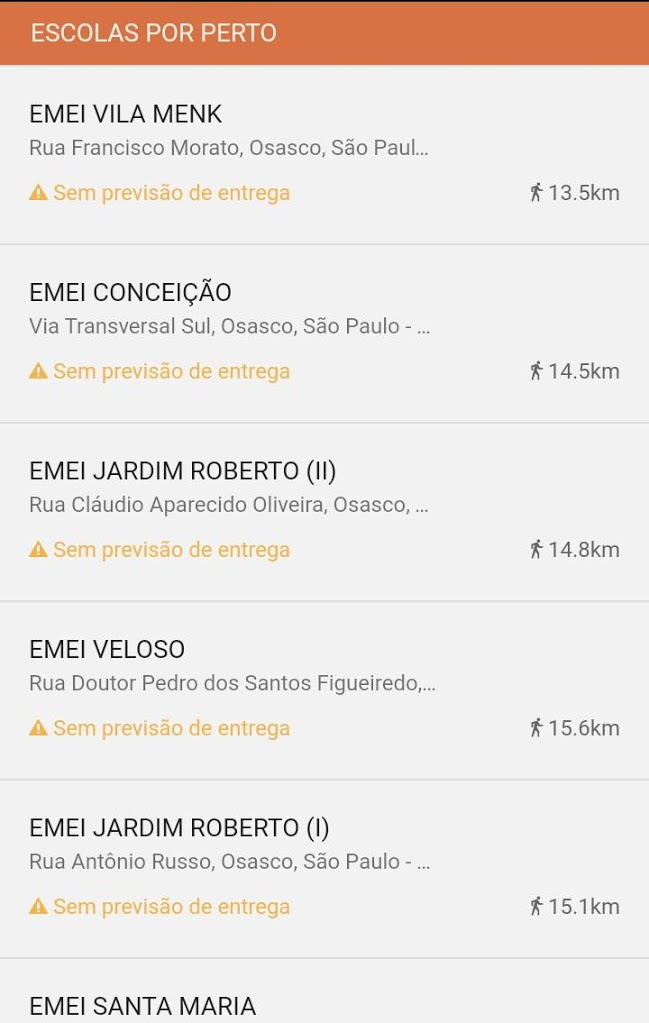
\includegraphics[scale=0.25]{tdp03.jpg}
       \label{}
     \end{minipage}
     \hfill
     \begin{minipage}[t]{.3\textwidth}
       \centering
       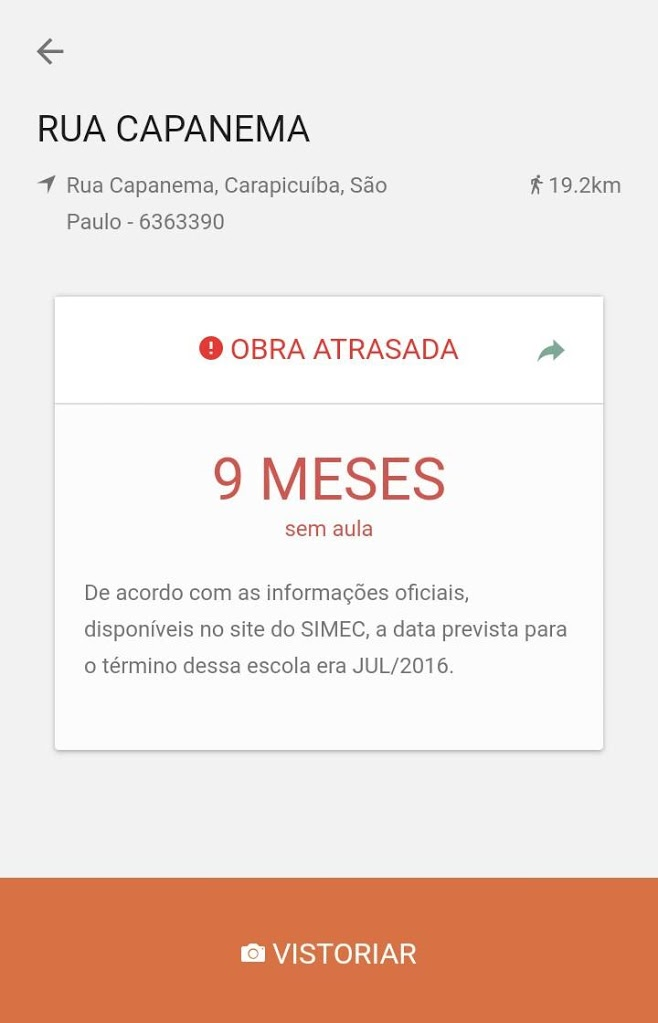
\includegraphics[scale=0.25]{tdp01.jpg}
     \end{minipage}
     \hfill
     \begin{minipage}[t]{.3\textwidth}
       \centering
       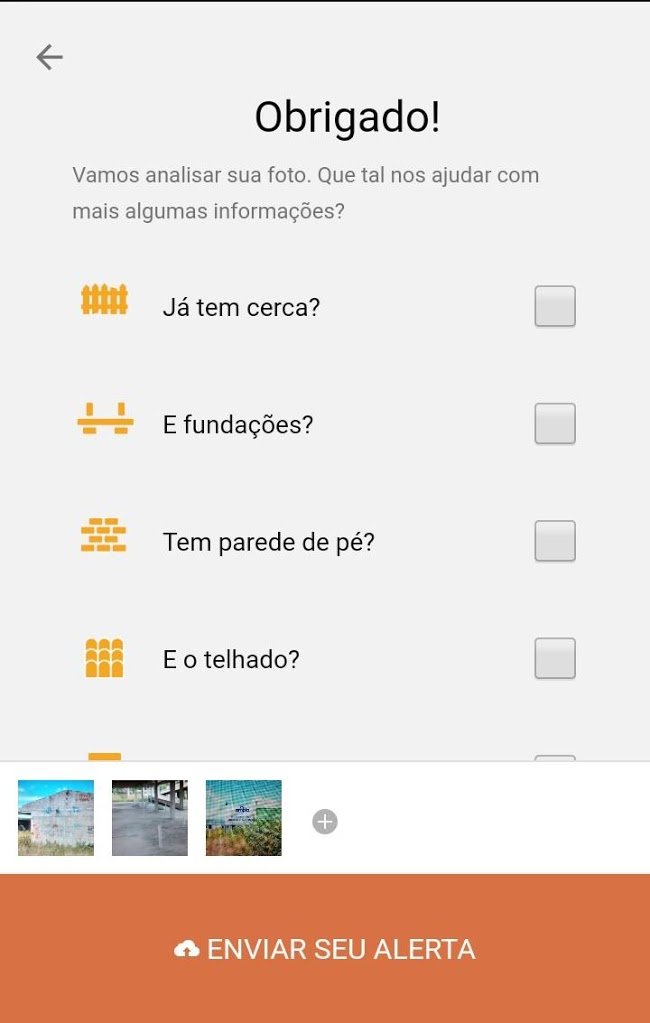
\includegraphics[scale=0.25]{tdp02.jpg}
     \end{minipage}
\caption{The \textit{Tá de Pé} mobile phone application. The first image presents a list of the closest school construction sites. The second image shows that a school construction is delayed by 9 months. The last image shows how citizens can add information to the photos they submit via the app.} 
\label{fig:screenshots}
\end{figure}

Transparência Brasil partnered with the Brazilian branch of
\emph{Engineers without Borders} (EWB), an independent non-governmental
organisation\footnote{Please visit
  \url{http://www.ewb-international.org} to know more about Engineers
  without Borders International and \url{https://esf.org.br} for
  information on the Brazilian office.}, to provide technical assessment
of school completion rates. The EWB bases their evaluations on photos
and GPS location sent through the app. The engineers' reports are later
uploaded to the database and stored on the users' mobile devices so
citizens can track the progress of the constructions.

The TDP has also received feedback from Brazilian computer programmers
and policy analists. In 2017 and 2018, Transparência Brasil announced
two team programming competitions, called `Tá de Pé Hackathons', where
contributors could fix code bugs and suggest new functionalities to the
TDP project. One of these innovations consists of a Twitter bot
(\url{https://twitter.com/tadepeapp}) which posts a message on the
social network each time a user submits a new picture for evaluation.
This allows interested parties to track the progress of construction
sites as well as add new public works to the TDP database.

\hypertarget{experimental-design}{%
\section{Experimental Design}\label{experimental-design}}

\label{sec:design}

Between August 2017 and August 2018, we implemented two interventions to
measure the effect of the TDP app on six school construction outcomes.
The outcomes are: 1) the percentage of public investment allocated to
school constructions; 2) the difference between the percentage invested
before and after the interventions; 3) the number of finished
constructions; 4) the number of cancelled constructions; 5) the number
of updated conclusion dates; 6) a placebo outcome indicating the
percentage of the investment executed before the impact evaluation
started. We expect the first five factors to increase the last one to
remain unchanged.

The first intervention was carried out from August 2017 to February 2018
using the Android version of the TDP app. The unit of analysis for this
experiment is the Brazilian municipality. We randomly selected 150
cities to the control group and included 1030 municipalities in the
treatment group. Our control condition consisted in removing all school
constructions in the chosen municipalities so that citizens were unable
to add information about them.

To evaluate the random assignment, we used the following pre-treatment
variables: 1) log of municipal population in 2015; 2) log of number of
poor families in each city; 3) log of total federal transfers to the
municipality in 2016; 4) federal government indicator for primary school
quality; 4) federal government indicator for secondary school quality.
The data come from the Brazilian Ministry of Education and the Census.
Balance tests show that the randomisation was successful and are
available in the Supplementary Materials.

We also conducted two manipulation checks and analysed the number of TDP
app downloads by municipality and app downloads over time. Figure
\ref{fig:manipulation1} displays the results. The checks display good
territorial variability. There were 455 downloads in the 1030
municipalities in the treatment condition. Downloads peak during the
Facebook TDP campaign, right after the TDP app launch in August, then
diminish over time. Please refer to the Supplementary Materials for a
detailed description of the tests.

\begin{figure}

{\centering \includegraphics[width=.49\linewidth]{article_files/figure-latex/man1-1} \includegraphics[width=.49\linewidth]{article_files/figure-latex/man1-2} 

}

\caption{\label{fig:manipulation1}Manipulation checks for intervention 1. The first plot shows the geographical distribution of the treatment condition and the second graph displays the number of TDP app downloads from August 2017 to February 2018.}\label{fig:man1}
\end{figure}

The second intervention is similar to intervention 1 in all but three
characteristics. First, the TDP app was available for Android and iOS
devices. Also, we randomised the intervention at the school level, with
654 control and 3895 treatment units. We used blocked randomisation
stratified by Brazilian state, school construction status (under
construction, stopped, unfinished) and whether the municipality spent
more on school construction that the distribution median. Finally, the
intervention period lasted from August 2018 to February 2019.

Balance tests and manipulation checks were also successful for
intervention 2. In total, 433 municipalities downloaded the app. There
is one download peak in August 2018, right after the intervention
starts, and a second spike around December. The number of downloads is
considerably smaller in this second intervention when compared to
intervention 1 as there was no associated social media campaign in that
period.

\begin{figure}

{\centering \includegraphics[width=.49\linewidth]{article_files/figure-latex/man2-1} \includegraphics[width=.49\linewidth]{article_files/figure-latex/man2-2} 

}

\caption{\label{fig:manipulation2}Manipulation checks for intervention 2. The graphs display the geographical and temporal variation of TDP app downloads from August 2018 to February 2019.}\label{fig:man2}
\end{figure}

We estimated all models using the following regression equation:

\[ Y_i \ = \ \alpha + \beta T_i + \gamma X_i + \theta Z_i + \varepsilon_i \]

where \(i\) indexes the experiment units. \(Y_i\) in one of the six
outcomes described above and \(\beta\) denotes the average treatment
effect. \(T_i\) is a binary treatment indicator, \(\gamma\) is a vector
of fixed effects, \(X_i\) is a matrix of Brazilian states' fixed
effects, \(\theta\) is a vector of controls and \(Z_i\) an array of
controls for the case \(i\). The error term is denoted by
\(\varepsilon_i\). We cluster the standard errors at the municipal level
as mayors are responsible for school investment decisions.

\hypertarget{results}{%
\section{Results}\label{results}}

\label{sec:results}

Table \ref{tab:results1} summarises the main results of intervention 1.
All models reported here include the five control variables described in
the previous section and Brazilian states' fixed effects. We also
estimated the models without control variables and fixed effects and the
results are unchanged. They are available in the Supplementary
Materials.

** TABLE 1 ABOUT HERE -- MAIN RESULTS INTERVENTION 1 **

\hypertarget{discussion}{%
\section{Discussion}\label{discussion}}

\label{sec:discussion}

\newpage
\setlength{\parindent}{0cm}
\setlength{\parskip}{5pt}

% More bibliography
\bibliography{references.bib}

\end{document}
